\documentclass{beamer}
\usepackage[english,russian]{babel}
\usepackage[utf8x]{inputenc}
\usepackage{graphicx} % для вставки картинок
\graphicspath{{res/}} % Путь к папке с картинками

% Математика
\usepackage{amssymb} % For use "mathbb" function
\usepackage{amsmath}
\usepackage{amsthm}
\usepackage{mathrsfs}
\newcommand{\La}{\mathscr{L}} % Функция Лагранжа
\newcommand{\ls}{{ℓ}} % Красивая l, чтобы легче было отличить от i, 1 b других палок
\providecommand{\norm}[1]{\lVert#1\rVert} % Норма вектора : ||w||
\newcommand{\dpt}[1]{\left\langle#1\right\rangle} % dot product using brackets
\newcommand{\brackets}[1]{\left(#1\right)} % Обернуть скобками автоматического размера
%\newcommand{\dpts}[2]{#2 \langle#1 #2 \rangle} % dot product using brackets with manual size
\newcommand{\R}{\mathbb{R}} % beautiful R for R^n labels
\newcommand{\il}{i = 1, \ldots, \ls} % writes i = 1, ..., l
\newcommand{\ili}{\quad i = 1, \ldots, \ls} % writes i = 1, ..., l with indent in begin
\newcommand{\sumil}{\sum_{i=1}^{\ls}} % Сумма по i, которая изменяется от 1 до l
\newcommand{\minl}{\min\limits} % min with limits under "min" label
\newcommand{\maxl}{\max\limits} % max with limits under "max" label

% Поправить стиль отрисовки формул (особенно актуально для сумм https://ru.sharelatex.com/learn/Display_style_in_math_mode)
\everymath{\displaystyle}

% Рисование схем
%\usepackage[all,cmtip]{xy}

% Стиль презентации
\usetheme{Warsaw}


% Добавление номеров для слайдов
%\useoutertheme{infolines}
\defbeamertemplate*{footline}{shadow theme}
{%
	\leavevmode%
	\hbox{\begin{beamercolorbox}[wd=.5\paperwidth,ht=2.5ex,dp=1.125ex,leftskip=.3cm plus1fil,rightskip=.3cm]{author in head/foot}%
			\usebeamerfont{author in head/foot}\insertframenumber\,/\,\inserttotalframenumber\hfill\insertshortauthor
		\end{beamercolorbox}%
		\begin{beamercolorbox}[wd=.5\paperwidth,ht=2.5ex,dp=1.125ex,leftskip=.3cm,rightskip=.3cm plus1fil]{title in head/foot}%
			\usebeamerfont{title in head/foot}\insertshorttitle%
		\end{beamercolorbox}}%
		\vskip0pt%
	}
	
% Окружение для определений
\AtBeginSection[]

\deftranslation{Definition}{Определение}

\beamertemplatenavigationsymbolsempty

\begin{document}
	\title[]{Фреймворк для конечно-разностного моделирования диффузионных задач на гибридных вычислительных кластерах}  
	\author{Фролов\,Д.\,A.}
	\institute{Ярославский государственный университет им. П. Г. Демидова \\ 
		\vspace{0.7cm}
		Научный руководитель:  Глызин\,С.\,Д. \\
		\vspace{0.7cm}
	}
	\date{Ярославль 2015} 
	% Создание заглавной страницы
	\frame{\titlepage} 
	% Автоматическая генерация содержания

\begin{frame}{Поставленная задача}
	Разработать программный комплекс для моделирования диффузионных задач.
	\begin{itemize}
		\item Вычислительное ядро
		\item Предварительная обработка
		\item Пользовательский интерфейс
	\end{itemize}
\end{frame}




\begin{frame}{Теоретические основы}
Общий вид задачи "<реакция-диффузия">
$$\frac{\partial u}{\partial t} = D \frac{\partial^2 u}{\partial x^2} + F(u);$$
$$\left.{\frac{\partial u}{\partial x}} \right|_{x=0} = \left.{\frac{\partial u}{\partial x}} \right|_{x=1} = 0, F(0) = 0.$$


Приближение оператора Лапласа его разностными аналогами

$$\left.{\frac{\partial^2 u}{\partial x^2}}\right|_{x=x_j} = \frac{u_{j-1} - 2u_j + u_{j+1}}{\bigtriangleup^2};$$
$$\dot u_j = D\, \frac{u_{j-1} - 2u_j + u_{j+1}}{\bigtriangleup^2} + F(u_j);$$
$$u_0 = u_1, u_{N+1} = u_N, j = \overline{1, N}.$$
\end{frame}






\begin{frame}{Пример области задачи}
	\begin{figure}[h]
		\center{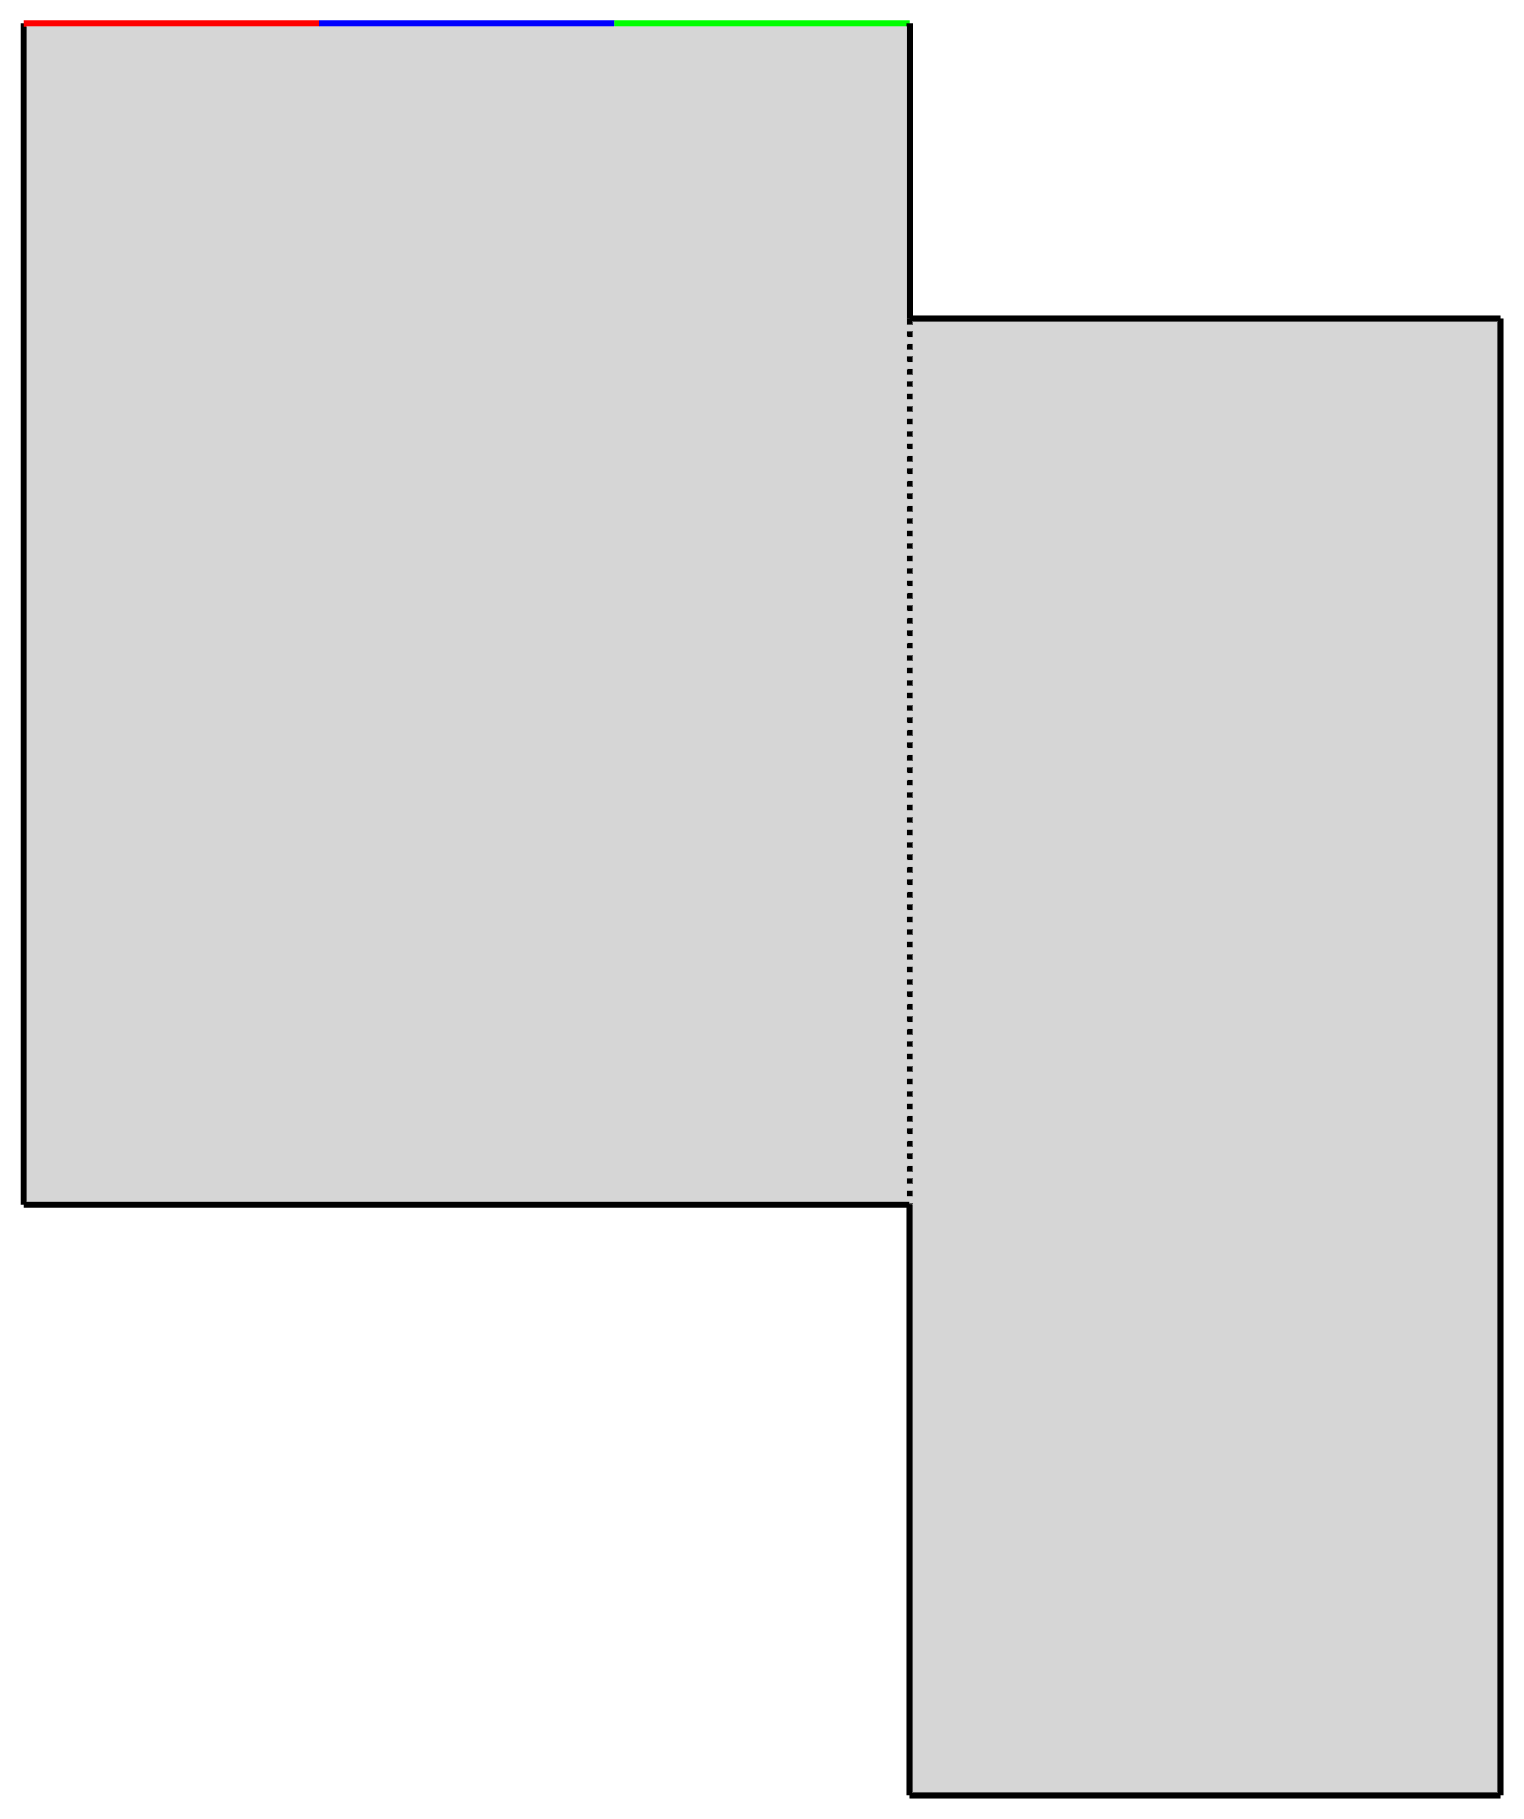
\includegraphics[width=0.7\linewidth]{2Block_ex.png}}
		\label{ris:2Block_ex}
	\end{figure}
\end{frame}






\begin{frame}{Класс Solver и его наследники}
	\begin{figure}[h]
		\center{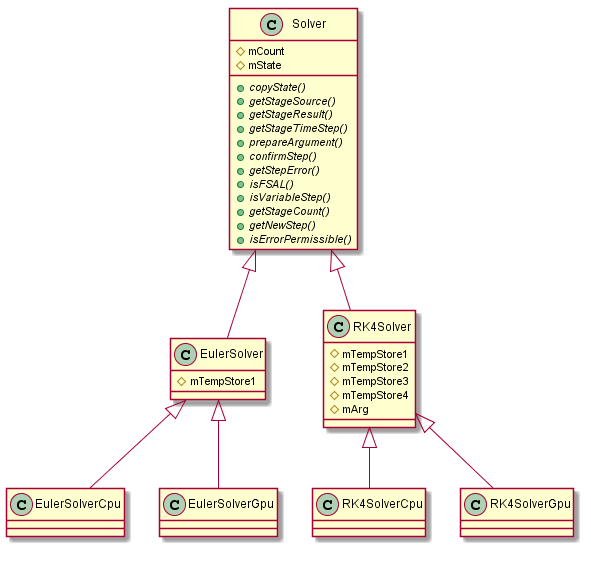
\includegraphics[width=0.7\linewidth]{solvers.png}}
		\label{ris:solvers}
	\end{figure}
\end{frame}




\begin{frame}{Класс Block и его наследники}
	\begin{figure}[h]
		\center{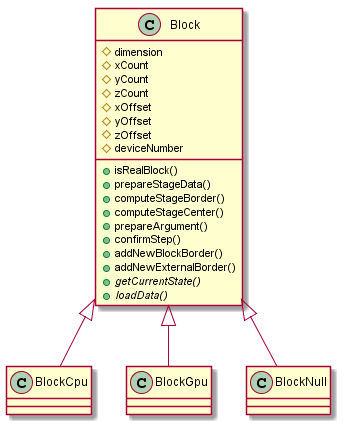
\includegraphics[width=0.6\linewidth]{blocks.png}}
		\label{ris:blocks}
	\end{figure}
\end{frame}





\begin{frame}{Общая схема классов приложения}
	\begin{figure}[h]
		\center{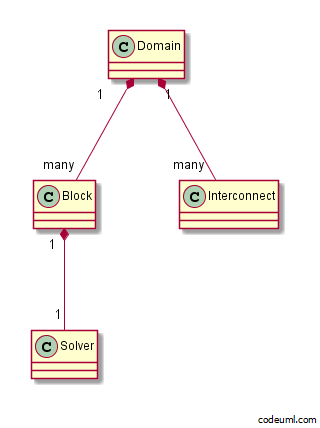
\includegraphics[width=0.6\linewidth]{all.png}}
		\label{ris:all}
	\end{figure}
\end{frame}






\begin{frame}{Параллельность}
	\begin{itemize}
		\item Крупнозернистый параллелизм -- разделение задачи на блоки
		\item Мелкозернистый параллелизм
		\begin{itemize}
			\item Центральный процессор -- OpenMP
			\item Видеокарта -- CUDA
		\end{itemize}
		
		\item Передача данных между узлами кластера -- библиотека MPI
	\end{itemize}
\end{frame}






\begin{frame}{Схема расчетов}
	\begin{figure}[h]
		\center{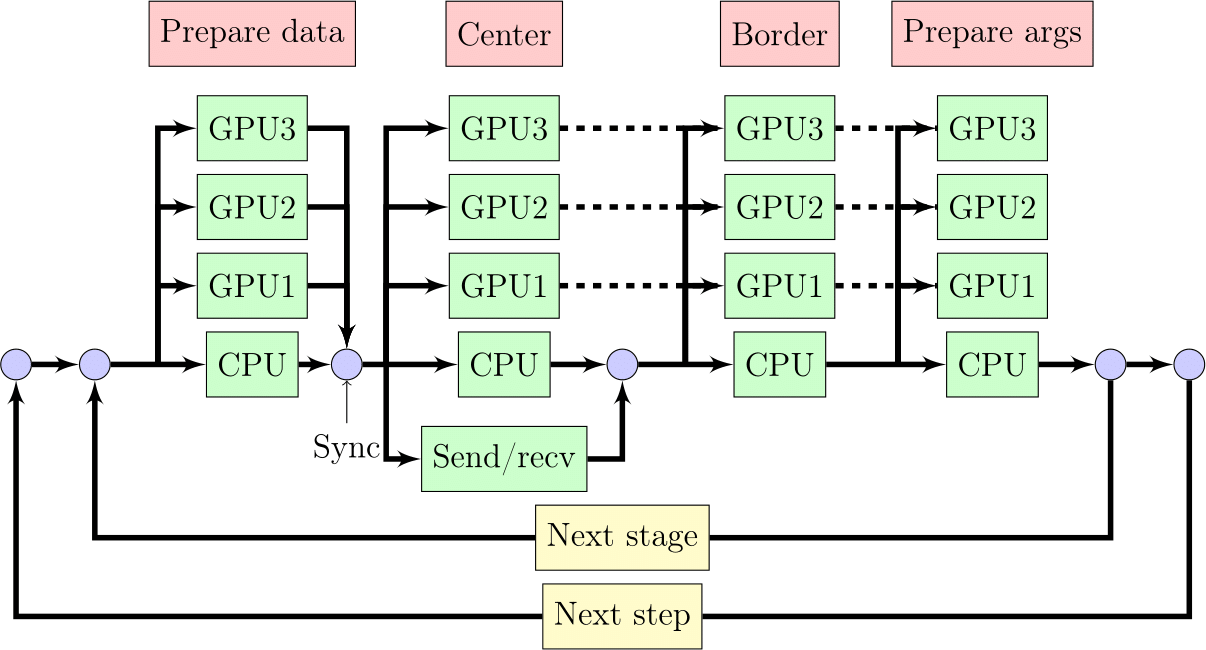
\includegraphics[width=1.0\linewidth]{scheme.png}}
		\label{ris:scheme}
	\end{figure}
\end{frame}





\begin{frame}{Результаты тестирования}
\center{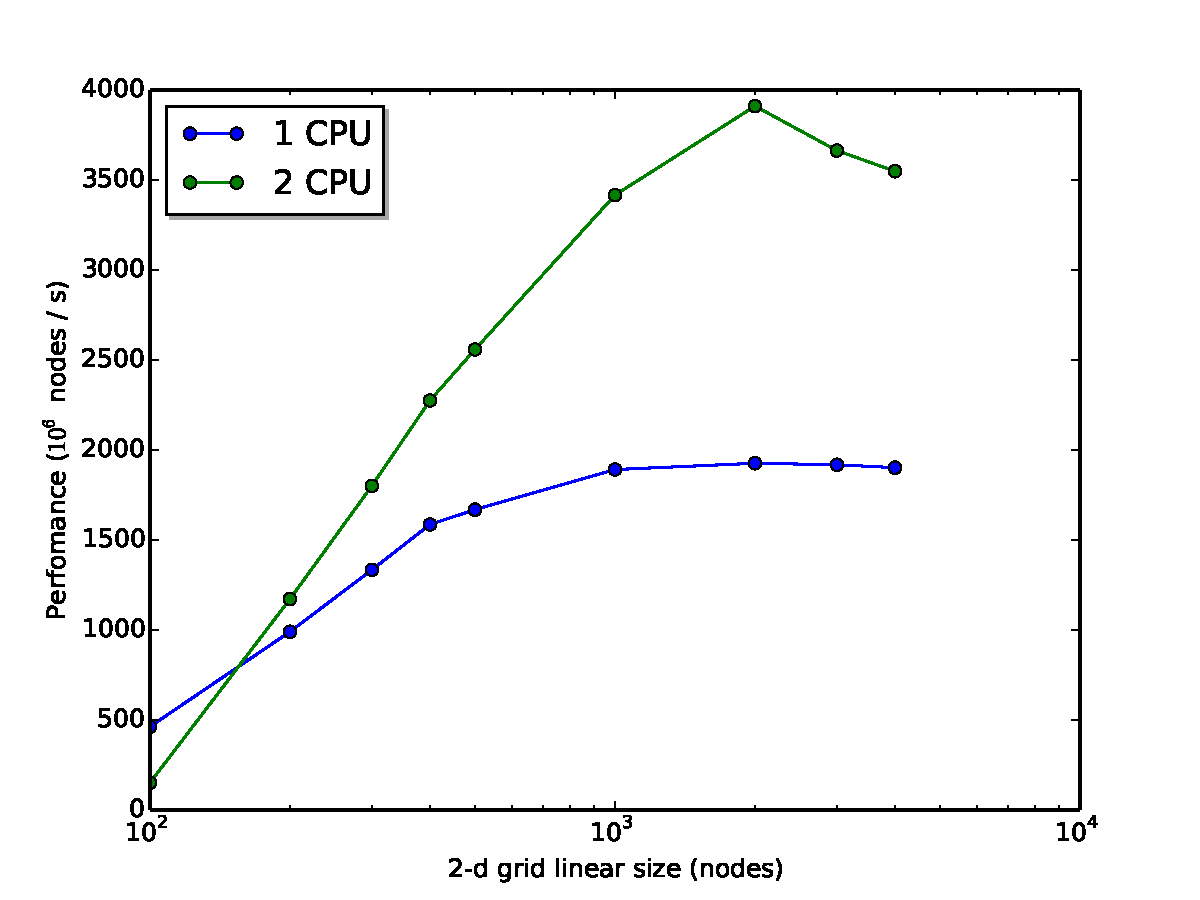
\includegraphics[scale=0.5]{CPU_1dev_2dev}}
\end{frame}

\begin{frame}{Результаты тестирования}
\center{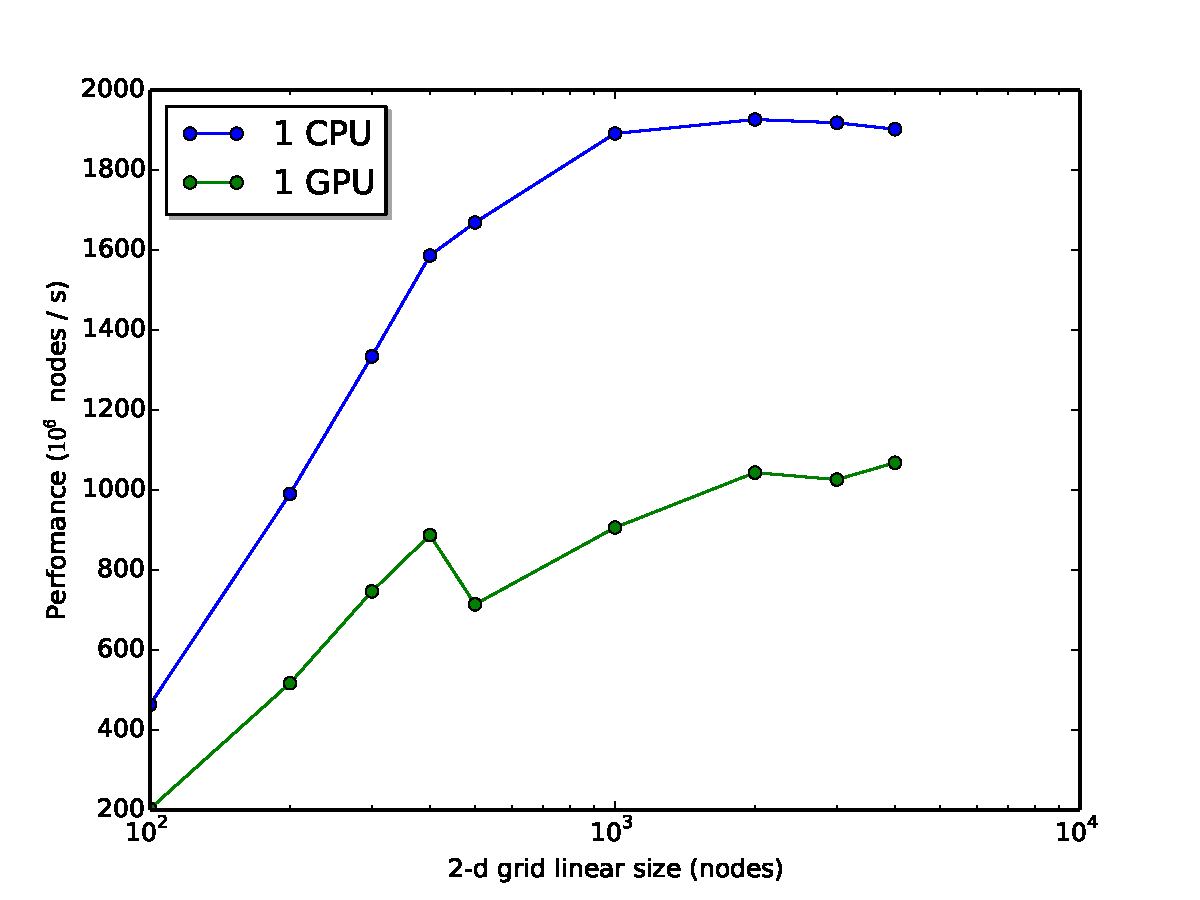
\includegraphics[scale=0.5]{CPU_GPU_1dev}}
\end{frame}

\begin{frame}{Результаты тестирования}
\center{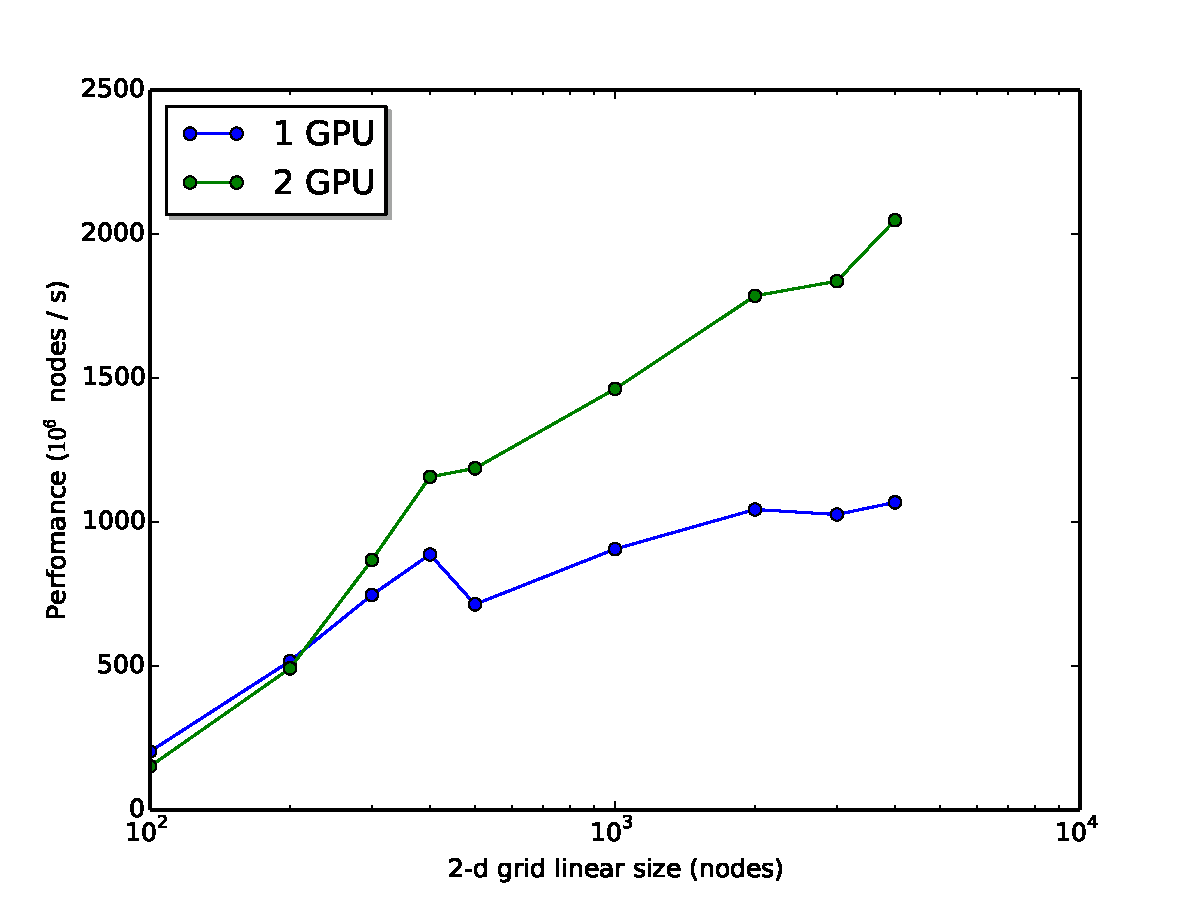
\includegraphics[scale=0.5]{GPU_1dev_2dev}}
\end{frame}

\begin{frame}{Результаты тестирования}
\center{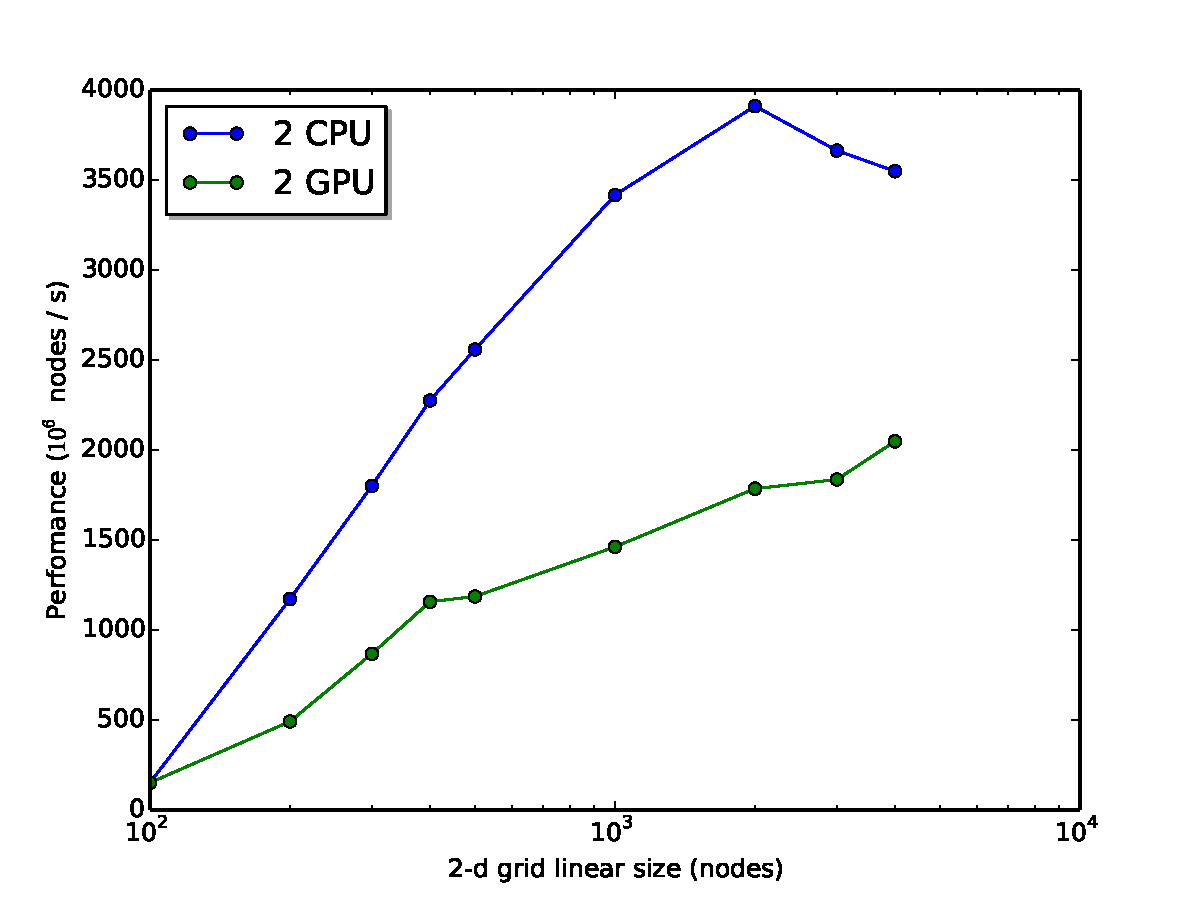
\includegraphics[scale=0.5]{CPU_GPU_2dev}}
\end{frame}

\begin{frame}{Результаты тестирования}
\center{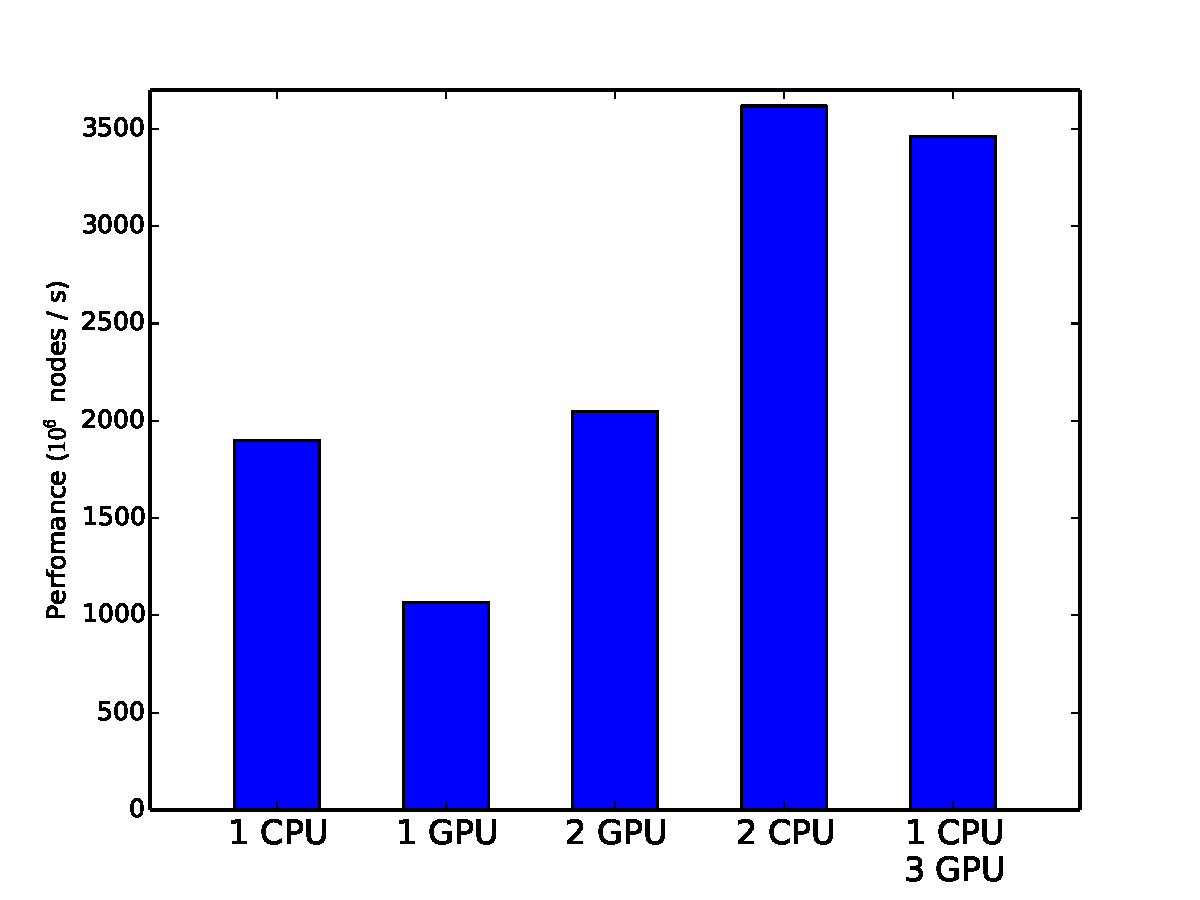
\includegraphics[scale=0.5]{hist}}
\end{frame}


\end{document}